%%%%%to do list %%%%%%

% 1. change arrow size in uni and bi directional pictures by using arrows.meta


%%%%%%%%%%%%%%%%%%%%%%%%%%%%%%%%%%%%%%
% LaTeX poster template
% Created by Nathaniel Johnston
% August 2009
% http://www.nathanieljohnston.com/2009/08/latex-poster-template/
%%%%%%%%%%%%%%%%%%%%%%%%%%%%%%%%%%%%%%

\documentclass[final]{beamer}
\usepackage{etex}
\usepackage{multicol}
\usepackage[scale=1.2]{beamerposter} 
\newcommand{\diag}{\mbox{{\rm diag}}}
\usepackage[labelformat=simple]{subcaption}
\renewcommand\thesubfigure{(\alph{subfigure})}
\captionsetup{compatibility=false}
\usepackage{pgfplots, graphicx, amsmath,amsthm,amssymb,mathtools,   natbib,tikz}

\usepackage{array}
\usepackage{booktabs}
\usetikzlibrary{arrows,snakes,backgrounds,shapes, decorations.markings}
\usetikzlibrary{matrix}
\usetikzlibrary{chains}
\usetikzlibrary{positioning}
\usetikzlibrary{arrows.meta, shadows, arrows, positioning}


%-----------------------------------------------------------
% Define the column width and poster size
% To set effective sepwid, onecolwid and twocolwid values, first choose how many columns you want and how much separation you want between columns
% The separation I chose is 0.024 and I want 4 columns
% Then set onecolwid to be (1-(4+1)*0.024)/4 = 0.22
% Set twocolwid to be 2*onecolwid + sepwid = 0.464
%-----------------------------------------------------------

\newlength{\sepwid}
\newlength{\onecolwid}
\newlength{\twocolwid}
\newlength{\threecolwid}
\setlength{\paperwidth}{48in}
\setlength{\paperheight}{36in}
%four columns settings
%\setlength{\sepwid}{0.024\paperwidth}
%\setlength{\onecolwid}{0.22\paperwidth}
%\setlength{\twocolwid}{0.464\paperwidth}
%\setlength{\threecolwid}{0.708\paperwidth}
%\setlength{\topmargin}{-0.5in}

%three columns settings
\setlength{\sepwid}{0.024\paperwidth}
\setlength{\onecolwid}{0.3013\paperwidth}
\setlength{\twocolwid}{0.626\paperwidth}
\setlength{\threecolwid}{0.626\paperwidth}
\setlength{\topmargin}{-0.5in}

%major theme colors
\usetheme{confposter}
\usepackage{exscale}
\usepackage{verbatim}
%\usepackage[linkcolor= blue]{hyperref} 
%-----------------------------------------------------------
% The next part fixes a problem with figure numbering. Thanks Nishan!
% When including a figure in your poster, be sure that the commands are typed in the following order:
% \begin{figure}
% \includegraphics[...]{...}
% \caption{...}
% \end{figure}
% That is, put the \caption after the \includegraphics
%-----------------------------------------------------------

\usecaptiontemplate{
\small
\structure{\insertcaptionname~\insertcaptionnumber:}
\insertcaption}

%-----------------------------------------------------------
% Define colours (see beamerthemeconfposter.sty to change these colour definitions)
%-----------------------------------------------------------

\setbeamercolor{block title}{fg=SFUred,bg=white}
\setbeamercolor{block body}{fg=black,bg=white}
\setbeamercolor{block alerted title}{fg=white,bg=SFUred}
\setbeamercolor{block alerted body}{fg=black,bg=SFUred!10}

%make sure figures are numbered
\setbeamertemplate{caption}[numbered]

%define theorem environments
\setbeamertemplate{theorems}[numbered]
\newtheorem{proposition}[theorem]{Proposition}

%-----------------------------------------------------------
% Name and authors of poster/paper/research
%-----------------------------------------------------------

\title{A Neural Network Approach to Classifying Banana Ripeness }
%\title{ \parbox[]{4in}{
\includegraphics[width=2.3in]{SFU_SocBlock-Horz_Pos_CMYK.eps}} \parbox[c]{33in}{A Neural Network Approach to Classifying Banana Ripeness} \parbox[c]{4in}{
\includegraphics[width=2.3in]{SFU_SocBlock-Horz_Pos_CMYK.eps} }}

\author{Kyle Demeule (kdd2@sfu.ca), Bernard S Chan (bernardc@sfu.ca), Saeed Soltani (saeeds@sfu.ca)}
\institute{Department Computing Science, Faculty of Applied Sciences, Simon Fraser University}

%-----------------------------------------------------------
% Start the poster itself
%-----------------------------------------------------------
\usepackage{gensymb}
\begin{document}
\begin{frame}[t]

  \begin{columns}[t]												% the [t] option aligns the column's content at the top
    \begin{column}{\sepwid}\end{column}			% empty spacer column
    \begin{column}{\onecolwid}
%      \begin{block}{Purpose}
%        Our purpose in this work is to investigate Hamiltonian coupled cell systems. Particularly, we are interested in the effects of coupling functions and coupling topology on the dynamics of the network. 
   %   \end{block}
      %\vskip2ex
\begin{block}{Introduction}
\begin{itemize}
\item Interested in classifying fruit ripeness using machine learning methods. 
\item Fruit ripeness has been studied previously through image segmentation methods~\citep{dadwal2012color}.
\item Banana ripeness was previously studied by~\citet{saad2009recognizing} and~\citet{paulraj2009color} through neural network methods. 
\item More than just bananas: aim to improve upon previous work by incorporating non-banana objects. 
\item Previous data set unavailable; will establish our own data set. 

\end{itemize}
\end{block} %introduction block
            \vskip2ex
\begin{alertblock}{Data Collection}
\begin{itemize}
\item Took pictures of bananas and non-banana objects.
\item Lighting, camera (Canon S90) and background were controlled. 
\item Used 12 unique bananas at various stages to represent the three stages ripeness: unripe, ripe and overripe. 
\item Non-banana objects: green pepper, apple, tomato, lemon, lime mushrooms, broccoli, potato and pears. 
\item Pictures were resized and cropped to $256\times256$. 
\item Incorporated each picture at $0\,^{\circ}$, $90\,^{\circ}$, $180\,^{\circ}$ and  $270\,^{\circ}$ of rotation to increase the number of pictures in the data set by four fold.
\item Total of 928 images generated. 
\end{itemize}
\end{alertblock}
 \vskip2ex
 \begin{figure}
 %%%%%% unripe %%%%%%%%%
  \begin{subfigure}{.123\textwidth}
  \centering
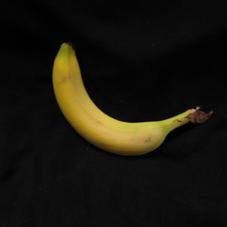
\includegraphics[width=\textwidth]{1_1.jpg}
\end{subfigure}%
 \begin{subfigure}{.123\textwidth}
  \centering
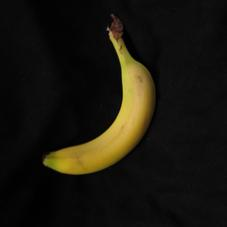
\includegraphics[width=\textwidth]{1_2.jpg}
\end{subfigure}%
  \begin{subfigure}{.123\textwidth}
  \centering
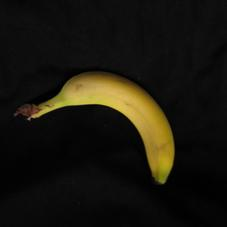
\includegraphics[width=\textwidth]{1_3.jpg}
\end{subfigure}%
  \begin{subfigure}{.123\textwidth}
  \centering
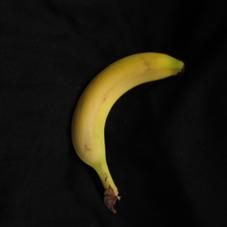
\includegraphics[width=\textwidth]{1_4.jpg}
\end{subfigure}\, %%%%%% ripe %%%%%%%%%
  \begin{subfigure}{.123\textwidth}
  \centering
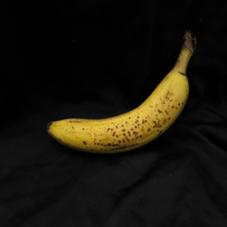
\includegraphics[width=\textwidth]{2_1.jpg}
\end{subfigure}%
 \begin{subfigure}{.123\textwidth}
  \centering
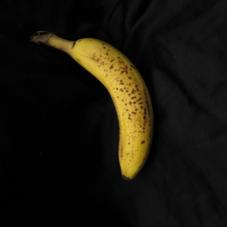
\includegraphics[width=\textwidth]{2_2.jpg}
\end{subfigure}%
  \begin{subfigure}{.123\textwidth}
  \centering
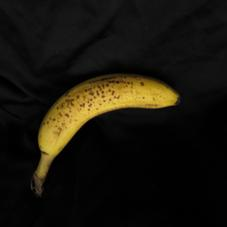
\includegraphics[width=\textwidth]{2_3.jpg}
\end{subfigure}%
  \begin{subfigure}{.123\textwidth}
  \centering
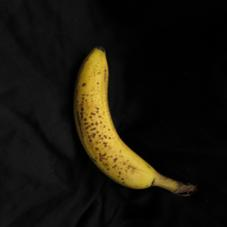
\includegraphics[width=\textwidth]{2_4.jpg}
\end{subfigure}%
\vskip .2in
 %%%%%% overripe %%%%%%%%%
  \begin{subfigure}{.123\textwidth}
  \centering
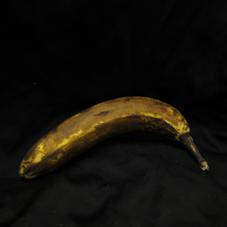
\includegraphics[width=\textwidth]{0_1.jpg}
\end{subfigure}%
 \begin{subfigure}{.123\textwidth}
  \centering
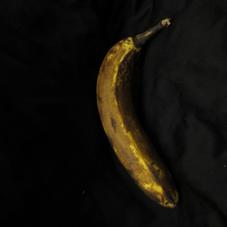
\includegraphics[width=\textwidth]{0_2.jpg}
\end{subfigure}%
  \begin{subfigure}{.123\textwidth}
  \centering
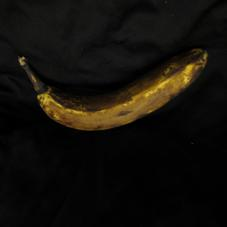
\includegraphics[width=\textwidth]{0_3.jpg}
\end{subfigure}%
  \begin{subfigure}{.123\textwidth}
  \centering
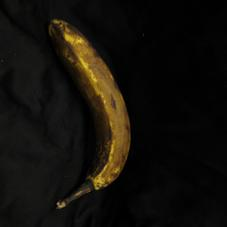
\includegraphics[width=\textwidth]{0_4.jpg}
\end{subfigure}\,
 %%%%%% non banana %%%%%%%%%
  \begin{subfigure}{.123\textwidth}
  \centering
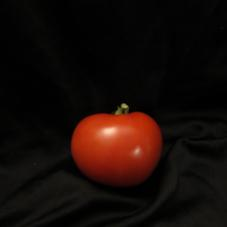
\includegraphics[width=\textwidth]{3_1.jpg}
\end{subfigure}%
 \begin{subfigure}{.123\textwidth}
  \centering
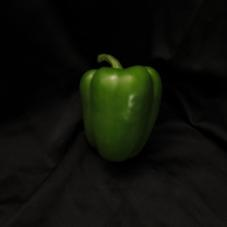
\includegraphics[width=\textwidth]{3_5.jpg}
\end{subfigure}%
  \begin{subfigure}{.123\textwidth}
  \centering
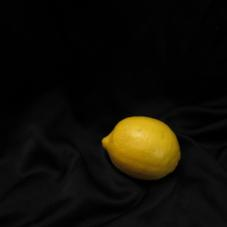
\includegraphics[width=\textwidth]{3_17.jpg}
\end{subfigure}%
  \begin{subfigure}{.123\textwidth}
  \centering
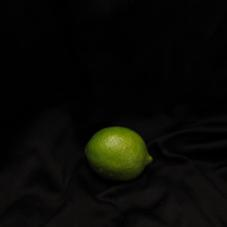
\includegraphics[width=\textwidth]{3_13.jpg}
\end{subfigure}%
\caption{Upper left: unripe bananas. Upper right: ripe bananas. Lower left: overripe bananas. Lower Right: non-banana objects.}
\end{figure}
\vskip1ex
\begin{block}{Methodology}
 \begin{itemize}
\item Extract features using pre-trained convolution neural network (CNN) from data set and classify them with support vector machine (SVM).
  \item Caffe~\citep{jia2014caffe}: deep learning framework for using AlexNet. 
 \item AlexNet~\citep{krizhevsky2012imagenet}: a pre-trained CNN for features extraction.
 \item SciKit Learn~\citep{scikit-learn}: a Python library of machine learning algorithms. 
 \begin{itemize}
 \item Applied C-Support Vector Classification (\emph{sklenar.svm.svc}) to the extracted features for classification. 
 \item Linear, RBF, sigmoid and polynomial kernels were compared. 
 \item Parameters optimization through exhaustive grid search (\emph{sklearn.grid\_search}).
 \end{itemize}
 \item Each set of four rotated pictures were either in the train or test set. 
  \item Workflow of this project is shown as a flowchart in Figure~\ref{fig:flowchart}
 \end{itemize}


  \end{block} %tools and methods block

\end{column}

    \begin{column}{\sepwid}\end{column}			% empty spacer column


        \begin{column}{\onecolwid}

          
 \begin{block}{Workflow}
\vskip-1ex
\tikzstyle{block} = [rectangle, draw, fill=SFUred!20, 
    text width=30em, text centered, rounded corners, minimum height=2em]
    \tikzstyle{small} = [rectangle, draw, fill=white!20, 
    text width=5em, text centered, rounded corners, minimum height=2em]
        \tikzstyle{medium} = [rectangle, draw, fill=white!20, 
    text width=8em, text centered, rounded corners, minimum height=2em]

\tikzstyle{line} = [draw, -latex']

\begin{figure}   
\centering 
\begin{tikzpicture}[node distance = 3.7cm, auto]
    % Place nodes
    \node [block] (capture) {Capture images};
    \node [block, below of=capture] (process) {Label and process images (crop, resize and convert to RGB)};
%    \node [block, below of=process] (convert) {Convert to RGB };
    \node [block, below of= process] (cnn) {Extract features via CNN (Caffe and AlexNet)};
    \node [block, below of=cnn] (svm) {Classify data via SVM (SciKit Learn)};
    \node [medium, below left = 2cm and -12cm of svm] (nonbanana) {Non-Banana};
    \node [small, below right = 2cm and -14 cm of svm] (banana) {Banana};
    \node [small, below of = banana] (ripe) {Ripe};
    \node [small, below left = 1.8 cm and 1.8 cm of banana] (unripe) {Unripe};
     \node [small, below right = 1.8cm and 1.8 cm of banana] (overripe) {Overripe};

    % Draw edges
    \path [line] (capture) -- (process);
    \path [line] (process) -- (cnn);
%    \path [line] (convert)--(cnn);
    \path [line] (cnn)--(svm);
    \path [line] (svm)--(nonbanana);
        \path [line] (svm)--(banana);
          \path [line] (banana)--(unripe);
        \path [line] (banana)--(overripe);
	\path [line] (banana)--(ripe);
\end{tikzpicture}
\caption{A flow chart of project development.}
\label{fig:flowchart}
 \end{figure}
  \end{block} %tools and methods block
         
%         \begin{theorem}\label{linearHamiltonianTheorem}
\vskip-1ex

\begin{alertblock}{Features Extraction via AlexNet}
\begin{figure}[h]
\centering
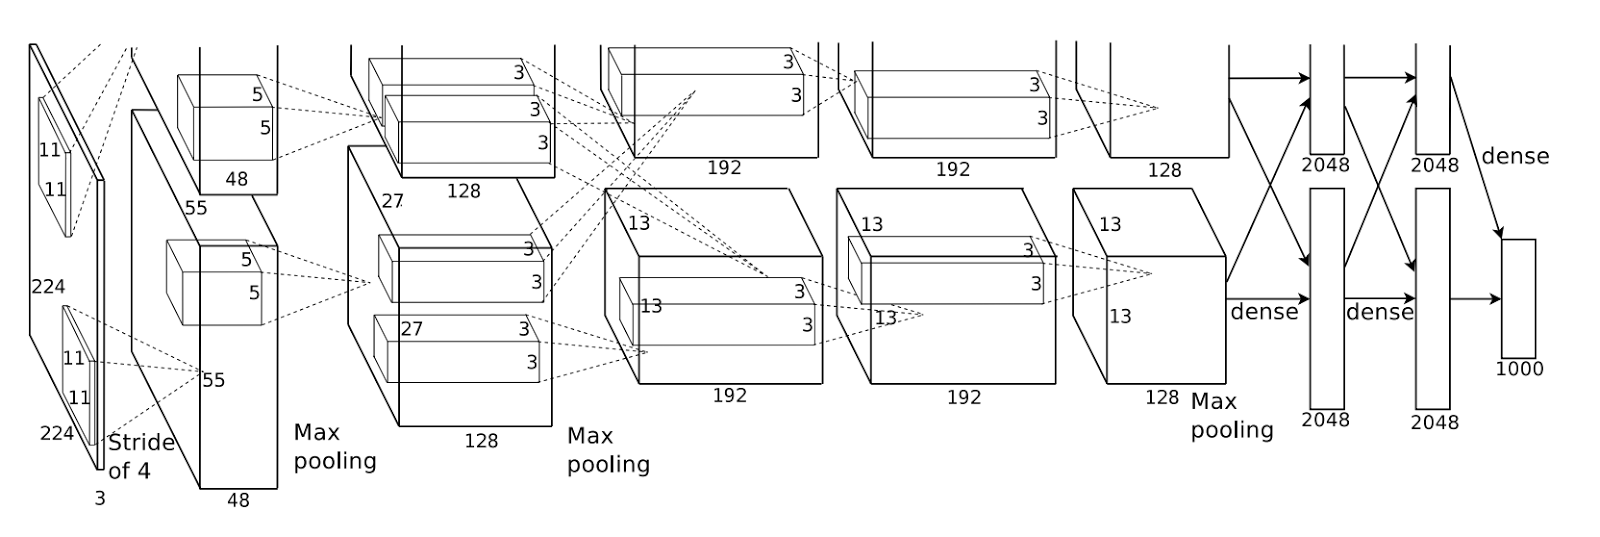
\includegraphics[width=\textwidth]{alexnet.png}
\caption{Architechture of AlexNet.}
\label{fig:alexnet}
\end{figure}
\vskip -1ex
\begin{itemize}
\item AlexNet: five convolutional layers and three fully connected layers.
\item Originally trained to classify images for the ILSVRC-2012 challenge. 
\item Extract representation of data set from last three layers (FC6, FC7 and FC8). 
\item Internal representations at these layers are vectors of length 4096 (FC6, FC7) or 1000 (FC8). 
\end{itemize}
\end{alertblock}

\begin{block}{Results}
\begin{itemize}
\item Tested various kernel methods from SciKit Learn's SVM library.
\item Experimental results are shown in Tables~\ref{tab:core} and~\ref{tab:banana}
\end{itemize}
\begin{table}[h]
\caption{Overall percentage of correctly classified objects from training and testing of SVM models with various kernels. Features were obtained from FC6, FC7 and FC8 exits of AlexNet. (Lin = linear, RBF = radial basis function, Sig = sigmoid, Poly = polynomial)}
\label{tab:core}
\begin{tabular}{|c|c|c|c|c|c|c|c|c|}\hline
 &  \multicolumn{4}{c|}{Training Results} & \multicolumn{4}{c|}{Testing Results}\\\hline
&Lin& RBF&Sig&Poly&Lin& RBF&Sig&Poly\\\hline
FC6&0.942&1.000&0.266&0.911&0.821&0.878&0.218&0.814\\\hline
FC7&0.876&1.000&0.266&0.872&0.788&0.862&0.218&0.804\\\hline
FC6&0.768&0.998&0.266&0.807&0.676&0.843&0.278&0.696\\\hline
\end{tabular}
\end{table}

\end{block}

 \end{column}
  \begin{column}{\sepwid}\end{column}			% empty spacer column        
  
        \begin{column}{\onecolwid}
        

%        \begin{theorem}
\begin{block}{Results}
\vskip -1ex

\begin{table}[h]
\small
\caption{Percentage of objects correctly classified based on banana, ripeness and non-banana objects. Features were obtained from FC6, FC7 and FC8 exits of AlexNet. (Lin = linear, RBF = radial basis function, Sig = sigmoid, Poly = polynomial)}
\label{tab:banana}
\begin{tabular}{|c|c|c|c|c|c|c|c|c|c|c|c|c|}\hline
 &  \multicolumn{4}{c|}{Banana as Banana} & \multicolumn{4}{c|}{Ripeness}& \multicolumn{4}{c|}{Object as Object}\\\hline
&Lin& RBF&Sig&Poly&Lin& RBF&Sig&Poly&Lin& RBF&Sig&Poly\\\hline
FC6&0.946&0.953&1.000&0.958&0.862&0.902&0.288&0.885&0.829&0.934&0.000&0.711\\\hline
FC7&0.924&0.945&1.000&0.932&0.885&0.901&0.288&0.895&0.697&0.882&0.000&0.711\\\hline
FC8&0.864&0.924&1.000&0.877&0.804&0.890&0.2880&0.826&0.618&0.908&0.000&0.605\\\hline
\end{tabular}
\end{table}

\vskip1ex

\begin{alertblock}{Results Summary}

\begin{itemize}
\item (RBF, FC6)  outperformed all other classifiers with 100.0\% accuracy in training and 87.8\% accuracy in testing.
\item (RBF, FC6) improved the performance of~\citet{saad2009recognizing} in classifying banana ripeness with significantly larger data set.
\item Sigmoid kernel classified every object as banana; 100\% accuracy in classifying banana but 100\% error on all non-banana objects.
\end{itemize}
\end{alertblock}

\end{block}
\begin{block}{Conclusion}
\begin{itemize}
\item Successfully enhanced previous work by adding non-banana objects. 
\item Future: generalize ripeness detection to other fruits and vegetables. 
\item Industrial application: automatic large scale sorting. 
\item Mobile app for visually disabled: find the ripeness of fruits and vegetables via phone camera. 
\item Code and data set available at \href{bit.ly/BananaRipe}{bit.ly/BananaRipe}
\end{itemize}
\end{block}
%\vskip1ex
\begin{block}{Acknowledgement}
We thank our TA Zhiwei (Lucas) Deng for his guidance on using Caffe as well as AlexNet and Dr. Mori for his insights on solving this problem. 
\end{block}
          \begin{block}{References}
   \bibliography{poster}		    
   \bibliographystyle{abbrvnat-no-title}
  \end{block}
  \vskip1ex
  \begin{figure}
  \centering
  
\includegraphics[width=.6\textwidth]{SFU_StdTag-Horz_Pos_CMYK.eps}
  \end{figure}
    \end{column}

 \end{columns}
\end{frame}
\end{document}
